\hypertarget{ariaid-title1}{%
\section{Context}\label{ariaid-title1}}

This section briefly explains the general context and the processes
using and impacted by LAM. This description reflects the situation to
date and may serve as a basis for deriving improvements.

EUR-Lex Legal Analysis Methodology (LAM) presents and describes the use
of metadata elements that are relevant for the legal and documentary
analysis of the EUR-Lex website's content.

The metadata elements employed in LAM are taken from the Common Data
Model (CDM) of the CELLAR repository of the Publications Office.

CELLAR is an electronic database which contains the documents and their
related metadata diffused on one of the websites of the Publications
Office. The CDM is an ontology that describes the concepts and
relationships (properties/elements) that can exist for the data stored
in the CELLAR.

LAM documentation contains descriptions of classes of legal documents
and a selection of metadata suitable for describing each document class.
LAM aims at facilitating the understanding and the use of relevant CDM
properties.

LAM gives some basic Definition for the metadata elements, determines
their cardinality and lists the related properties. It also gives some
methodological rules concerning the use of the elements in different
contexts during the legal analysis. It also describes which kind of data
has to be used when filling in the metadata elements. If a metadata
element has to be completed with a value coming from a controlled
vocabulary, it is indicated. If there is no indication, it means that
the metadata element can be filled in with free text.

The process involving LAM starts with the legal documents (LD) published
in CELLAR. Then the legal analysis team receives an XML Notice and
access to the HTML content. At this stage, the notice contains a minimal
set of metadata which may or may not be correct.

The goal is to (a) verify the correctness of the existing metadata, (b)
classify the document according to LAM methodology (c) enrich the
document with the corresponding legal metadata.

The document classification, for instance, is performed by considering
the structure of the document title (i.e. presence/absence of keywords),
structure of the CELEX number (if present), author and other metadata.
For example, the title which contains string "communication of the
commission" required that the author is the European Commission (EC) and
is classified as a certain LAM document class.

Enrichment of the corresponding legal metadata is manually performed
under the guidance of the LAM documentation.

The diagram below depicts operations performed using the published Legal
Document and the XML notice \& metadata. Document classification,
validation of publishing metadata and enrichment with legal metadata are
performed by an external contractor. The legal analysis team further
performs a quality control of the legal document and XML notice and
metadata and ensure the dissemination of the metadata dissemination on
EuroLex website and other channels.

\begin{figure}
\centering
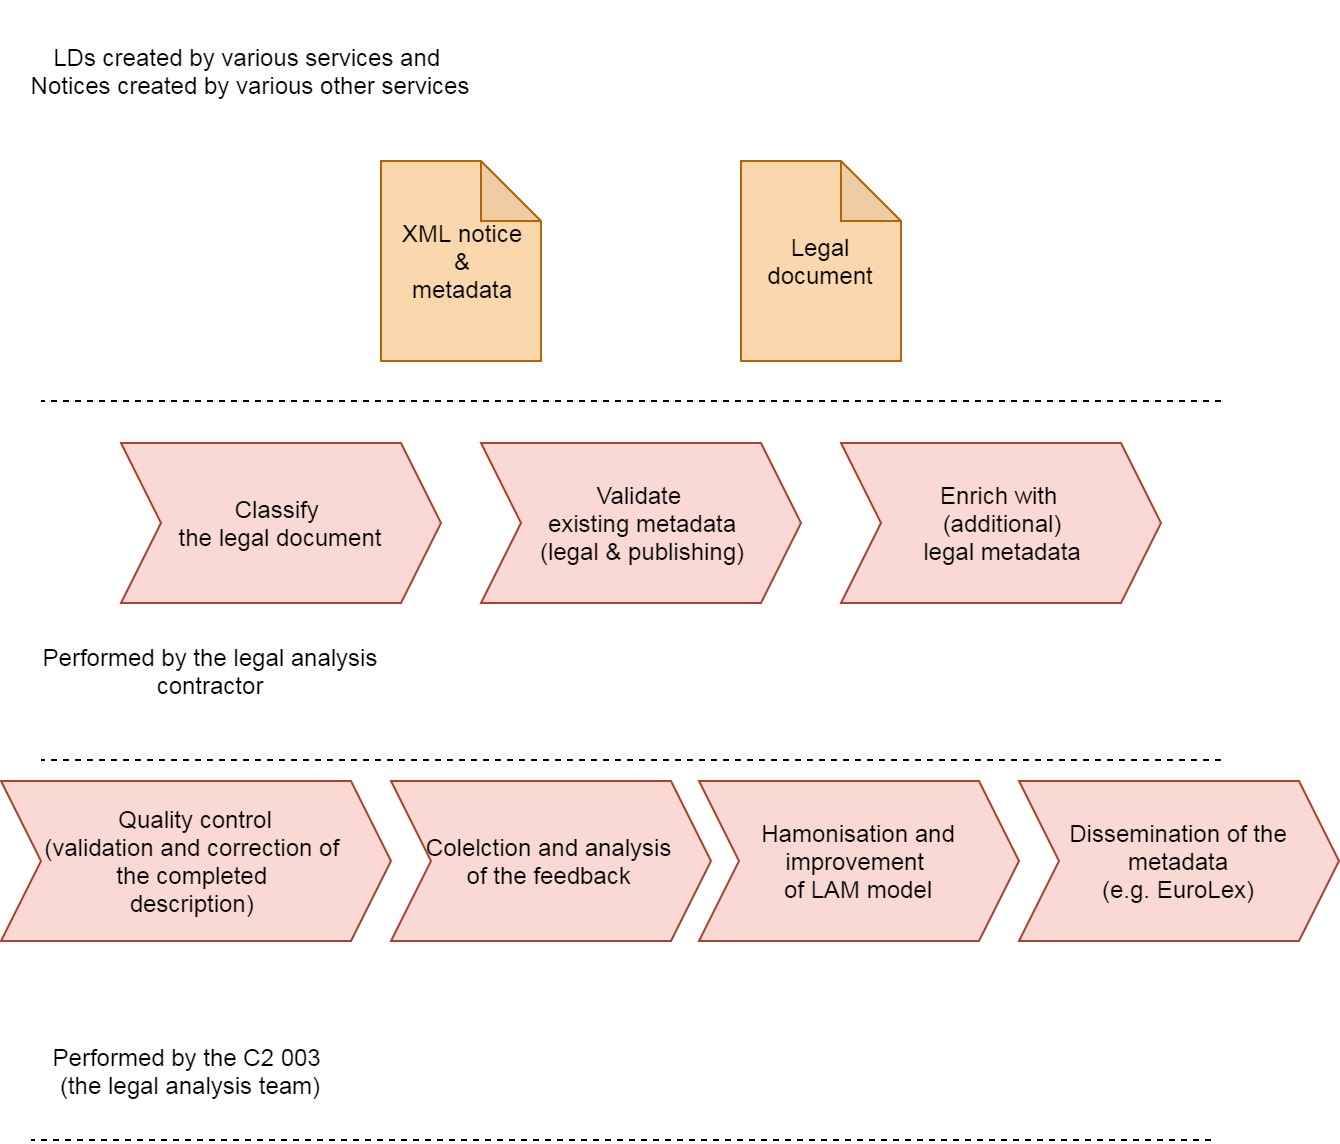
\includegraphics[width=5in,height=\textheight]{../../docs/LAM context.jpg}
\caption{{Figure{ 1}: }Digital assets and operations related to legal
analysis methodology}
\end{figure}

In addition, the legal analysis team is the LAM owner and main editor.
This role implies collecting feedback from various stakeholders and
partners; initiating projects to harmonise and improve the quality of
LAM itself.
